\chapter{Cascading Verification}
\label{chap:Cascading_Verification}

Cascading verification combines the technologies described in Chapter~\ref{chap:Domain_Modeling} to enhance the abstraction level of model and property specifications, and the effectiveness of probabilistic model checking; our prototype implementation of cascading verification combines these technologies to support the probabilistic verification of UAV mission plans. This chapter describes the prototype by tracing verification from high-level mission specifications to probabilistic model checking with PRISM\@. As with Chapter~\ref{chap:Domain_Modeling}, cascading verification is illustrated with respect to Mission~A, the example mission presented in Section~\ref{sec:An_Example_Mission}.

The remainder of this chapter is structured as follows. Section~\ref{sec:High_Level_Specifications_in_YAML} presents the YAML DSL used by model builders to encode mission plans and the geographic data associated with those plans. Section~\ref{sec:Verification_with_Semantic_Reasoning} describes the transformation of mission specifications into ABox assertions, and the verification of those assertions via automated semantic reasoning. Section~\ref{sec:Verification_with_Semantic_Reasoning} also describes inferred ontological knowledge, which is generated via automated reasoning from explicitly encoded domain knowledge. Section~\ref{sec:Classification_with_Prolog} describes the transformation of explicit and inferred ontological knowledge into Prolog facts, and the Prolog inferences resulting from those facts. Explicit domain knowledge---encoded in OWL+SWRL and Prolog---and knowledge inferred via composite reasoning is used by our prototype to synthesize DTMC and PCTL artifacts, which are presented in Section~\ref{sec:Synthesized_Models_and_Properties}. This section also presents results from the probabilistic model checking underpinned by synthesized artifacts. The technologies and implemented components that constitute our prototype are presented in Section~\ref{sec:Implementation}. Our work is related to semantic model checking, which is presented in Section~\ref{sec:Cascading_Verification_Related_Work}. This chapter is summarized in Section~\ref{sec:Cascading_Verification_Summary}.

\section{High-Level Specifications in YAML}
\label{sec:High_Level_Specifications_in_YAML}

With cascading verification, model builders use a DSL to encode high-level system specifications. In the context of our prototype, model builders use YAML to encode mission plans and the geographic data associated with those plans. The prototype comprises a domain-specific YAML dialect that is consistent with the domain concepts formalized in CEMO\@. Consistency is enforced when mission specifications are transformed by the CVC into ABox assertions, and verified via semantic reasoning with respect to the TBox defined by domain experts.

To better illustrate the YAML DSL, which specifies Mission~A, we have encoded a schema definition in the Kwalify schema language~\cite{Kuwata_2011}. This schema is partially defined in Listing~\ref{lst:partial_schema_definition}.

\begin{figure}[ht]
\begin{lstlisting}[caption={Partial schema definition for the YAML DSL},label=lst:partial_schema_definition]
type: map
required: yes
mapping:
  "Action":
    type: map
    required: yes
    mapping:
      "HoverAction":
      (*\ldots*)
      "LidarAction":
      (*\ldots*)
      "PhotoSurveillanceAction":
      (*\ldots*)
      "TraversePathSegmentAction":
      (*\ldots*)
  "Asset":
    type: map
    required: yes
    mapping:
      "ARDrone":
      (*\ldots*)
      "Hummingbird":
      (*\ldots*)
\end{lstlisting}
\end{figure}

The Kwalify schema language is itself a dialect of YAML\@. Lines~1--3 in Listing~\ref{lst:partial_schema_definition} declare a YAML mapping, which is a primary logical structure in a YAML document (lines~5--7 and~17--19 declare similar data structures). The Kwalify keyword \texttt{required} is used in lines~2, 6 and~18 to denote constraints on each of the declared mappings.

According to Listing~\ref{lst:partial_schema_definition}, the YAML DSL affords mission developers two top-level elements---\texttt{Action} and \texttt{Asset} (declared in lines~4 and~16, respectively)---that must be specified for each mission. The former contains four optional elements---\texttt{HoverAction}, \texttt{LidarAction}, \texttt{PhotoSurveillanceAction} and \texttt{TraversePathSegmentAction} (declared in lines~8--14)---while the latter contains optional elements \texttt{ARDrone} and \texttt{Hummingbird} (declared in lines~20 and~22, respectively). The YAML code in Listing~\ref{lst:DSL_element_Hummingbird} specifies the DSL element \texttt{Hummingbird}.

\begin{figure}[ht]
\begin{lstlisting}[caption={Schema definition for the DSL element \texttt{Hummingbird}},label=lst:DSL_element_Hummingbird]
"Hummingbird":
  type: seq
  sequence:
    - type: map
      required: yes
      mapping:
        "id":
          type: int
          required: yes
        "endurance":
          type: int
        "actions":
          type: seq
          required: yes
          sequence:
            - type: int
\end{lstlisting}
\end{figure}

Lines~2 and~3 in Listing~\ref{lst:DSL_element_Hummingbird} declare a YAML sequence, which is a primary logical structure in a YAML document (lines~13--15 declare a similar data structure). According to Listing~\ref{lst:DSL_element_Hummingbird}, the element \texttt{Hummingbird} contains the required element \texttt{id} and the optional element \texttt{endurance} (declared in lines~7 and~10, respectively), both of which assume values of type \texttt{int}. The element \texttt{Hummingbird} also contains the required element \texttt{actions} (declared in line~12), which is a sequence of \texttt{int} values that identify actions assigned to a specific \texttt{Hummingbird} asset. The elements \texttt{actions} and \texttt{endurance} correspond, respectively, to the object property \texttt{hasAction} and the datatype property \texttt{hasEnduranceInSeconds} encoded in Listing~\ref{lst:OWL_class_Asset}.

Appendix~\ref{chap:DSL_Schema} presents a complete schema definition for the YAML DSL\@.

\section{Verification with Semantic Reasoning}
\label{sec:Verification_with_Semantic_Reasoning}

Mission specifications encoded in YAML are transformed by the CVC into ABox assertions. During this preprocessing phase, geodesic equations use geographic coordinates (described in Section~\ref{sec:An_Example_Mission}) and threat area data from external sources to calculate supplementary geographic information. For example, if the boundary of a threat area is intersected by a flightpath, then the traverse path segment action corresponding to that flightpath is classified as a threat area action. Geodesic equations can be used to establish threat area incursions in this manner because both flightpath and threat area boundary are defined by \emph{great circles}.\footnote{A great circle is the intersection of the Earth's surface with a plane passing through the center of the Earth. The concepts that underpin geodesic equations will be elaborated in Appendix~\ref{chap:Threat_Area_Calculations}.}

Pellet verifies the generated ABox against the TBox defined by domain experts. Inconsistencies between TBox and ABox signify an invalid mission specification; for example, an asset that does not execute at least one kinetic action would be inconsistent with respect to the definition of class \texttt{Asset} presented in Section~\ref{sec:Semantic_Modeling}. The OWL code in Listing~\ref{lst:OWL_individual_H1} formally defines a valid ABox individual with identifier~\texttt{H1}, which corresponds to the identifier of the Hummingbird asset specified in Mission~A.

\begin{figure}[ht]
\begin{lstlisting}[caption={OWL code for the individual \texttt{H1}},label=lst:OWL_individual_H1]
Individual: H1
  Types: Hummingbird
  Facts: hasAction TPSA1,
    hasAction TPSA2
\end{lstlisting}
\end{figure}

Asset~\texttt{H1} is related via the object property \texttt{hasAction} to actions~\texttt{TPSA1} and~\texttt{TPSA2} (lines~3 and~4, respectively, in Listing~\ref{lst:OWL_individual_H1}). Mission~A specifies that action~\texttt{TPSA1} is a precondition to action~\texttt{TPSA2} (line~10 in Listing~\ref{lst:Mission_A}). Because preconditions associate actions with other actions, a precondition would be inconsistent, with respect to the definition of the object property \texttt{hasPrecondition} presented in Section~\ref{sec:Semantic_Modeling}, if it associated individuals that were not members of class \texttt{Action}. The OWL code in Listing~\ref{lst:OWL_individuals_TPSA1_TPSA2} specifies two valid ABox individuals with identifiers~\texttt{TPSA1} and~\texttt{TPSA2}, where~\texttt{TPSA2} is related to~\texttt{TPSA1} via \texttt{hasPrecondition} (line~6). Figure~\ref{fig:semantic_verification} illustrates elements of semantic verification with respect to the actions \texttt{TPSA1} and \texttt{TPSA2}, and the object property \texttt{hasPrecondition}. As a valid ABox individual, action \texttt{TPSA2} inherits from the built-in OWL class \texttt{Thing}, which is highlighted with red text (an invalid individual would inherit from the built-in OWL class \texttt{Nothing}).

\begin{figure}[ht]
\begin{lstlisting}[caption={OWL code for the individuals \texttt{TPSA1} and \texttt{TPSA2}},label=lst:OWL_individuals_TPSA1_TPSA2]
Individual: TPSA1
  Types: TraversePathSegmentAction

Individual: TPSA2
  Types: TraversePathSegmentAction
  Facts: hasPrecondition TPSA1
\end{lstlisting}
\end{figure}

\begin{figure}[ht]
\centering
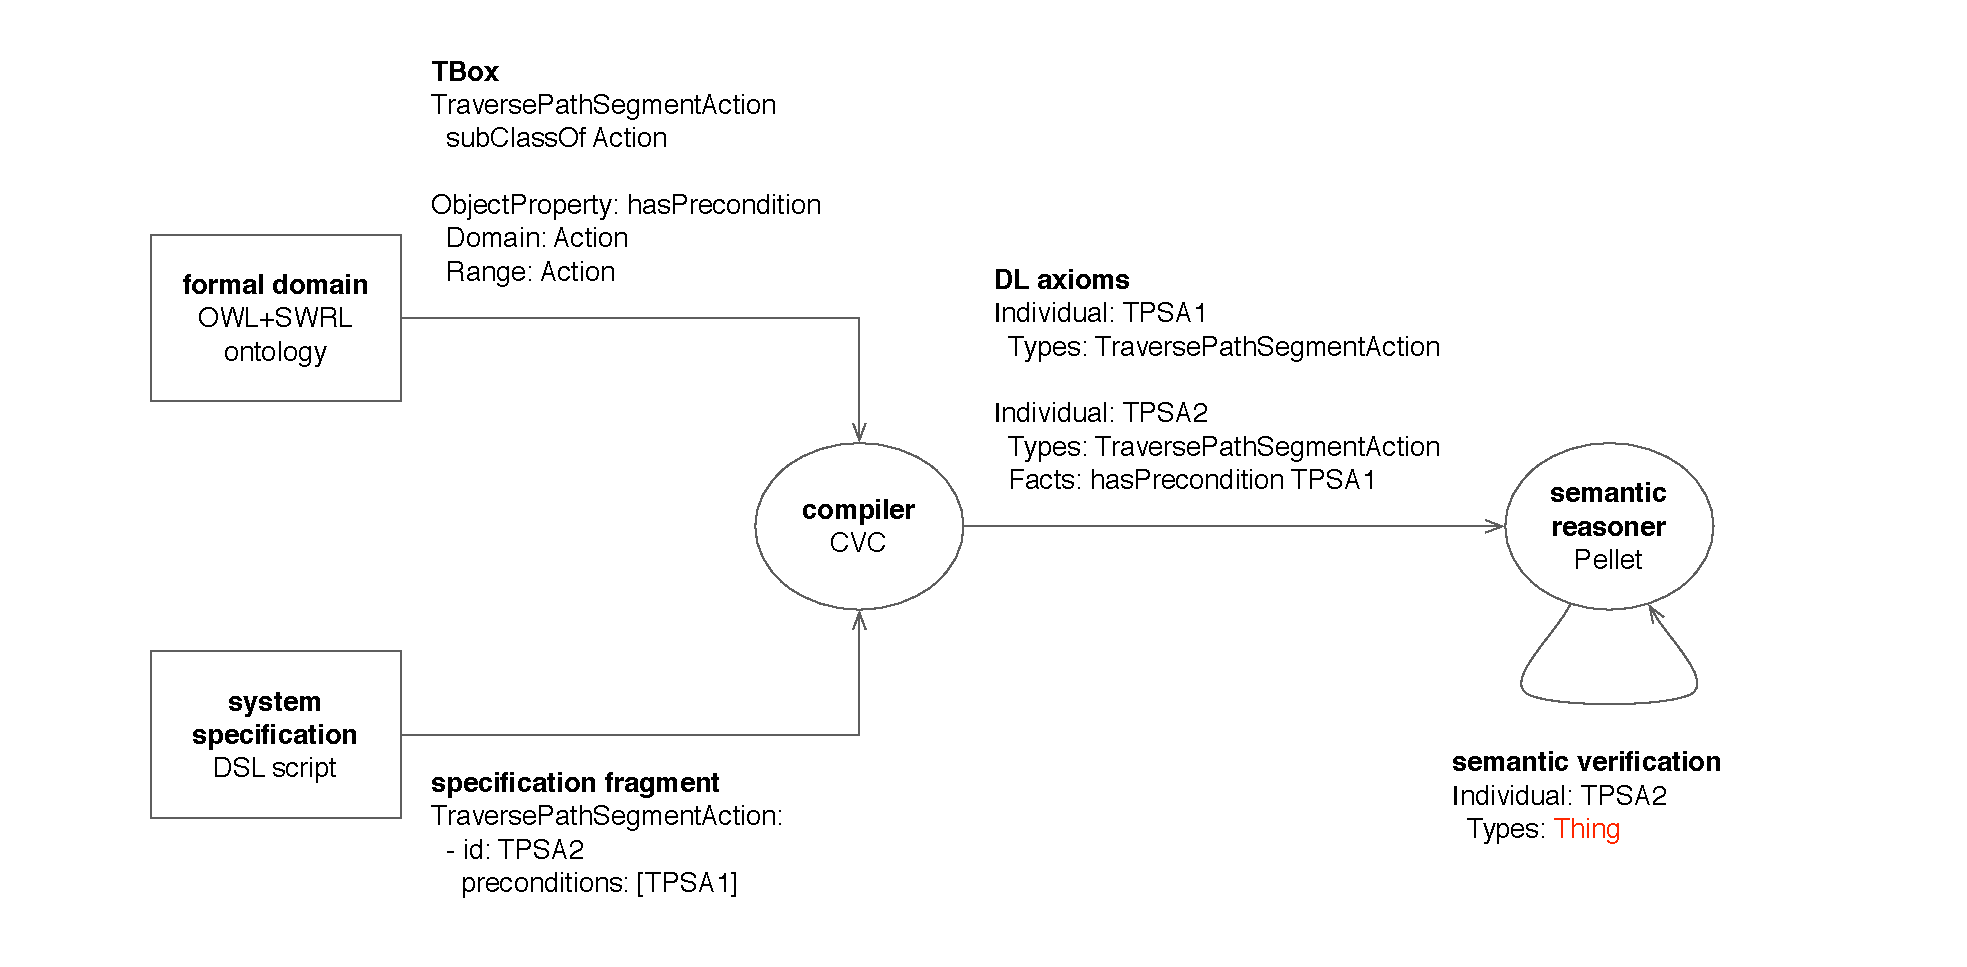
\includegraphics[width=\textwidth]{img/semantic-verification.pdf}
\caption[Semantic verification]{Elements of semantic verification with respect to the actions \texttt{TPSA1} and \texttt{TPSA2}, and the object property \texttt{hasPrecondition}.}
\label{fig:semantic_verification}
\end{figure}

With ABox consistency deduced, Pellet proceeds to generate inferences by, for example, reasoning about \emph{realization}, which determines the direct types of each individual. Realization-based inferences were described in Section~\ref{sec:Modeling_Tactical_Missions} with the classification of a specific kinetic action as a DTAA, and the resultant classification of the asset to which that action was assigned as a valid asset. As an example of realization with respect to Mission~A, let us assume a threat area action classification for action \texttt{TPSA4} (via the preprocessing phase described above). Given this assumption, Pellet would infer action \texttt{TPSA4} to be a DTAA because start point and endpoint of \texttt{TPSA4} are members of classes \texttt{Waypoint} (the start point of action \texttt{TPSA4} is the endpoint of action \texttt{TPSA3}, which is not a threat area action) and \texttt{ThreatAreaWaypoint}, respectively. Asset~\texttt{H2} would consequently be inferred a valid asset (since~\texttt{H2} executes at least one sensor action, namely \texttt{PSA5}, during the incursion).

Appendix~\ref{chap:Ontology} presents the generated ABox for Mission~A.

\section{Classification with Prolog}
\label{sec:Classification_with_Prolog}

Some Pellet inferences are transformed by the CVC into Prolog rules; for example, the Prolog rule \texttt{terminal} comprises knowledge inferred by Pellet (as described in Section~\ref{sec:Rule_Based_Modeling}). The Prolog code in Listing~\ref{lst:Prolog_rule_terminal_constrained_observer} formally defines rule \texttt{terminal\_constrain\-ed\_observer}, which encapsulates the atom \texttt{terminal}.

\begin{figure}[ht]
\begin{lstlisting}[caption={Prolog code for rule \texttt{terminal\_constrained\_observer}},label=lst:Prolog_rule_terminal_constrained_observer]
terminal_constrained_observer(X) :-
  constrained_observer(X),
  terminal(X).
\end{lstlisting}
\end{figure}

SWI-Prolog classifies each kinetic action with respect to the relationships that exist between it and other kinetic actions. For example, an action that is the last kinetic action to be executed by an asset, and has as precondition at least one cross-cutting kinetic action, is classified by SWI-Prolog as a \texttt{terminal\_constrained\_observer} (cross-cutting actions were introduced in Section~\ref{sec:Rule_Based_Modeling}). Figure~\ref{fig:composite_reasoning} illustrates elements of composite semantic- and Prolog-based reasoning with respect to the actions \texttt{TPSA1} and \texttt{TPSA2}; the inferred object property \texttt{isPreconditionTo} presented in Section~\ref{sec:Rule_Based_Modeling}; and the rule \texttt{terminal\_constrained\_observer}.

\begin{figure}[ht]
\centering
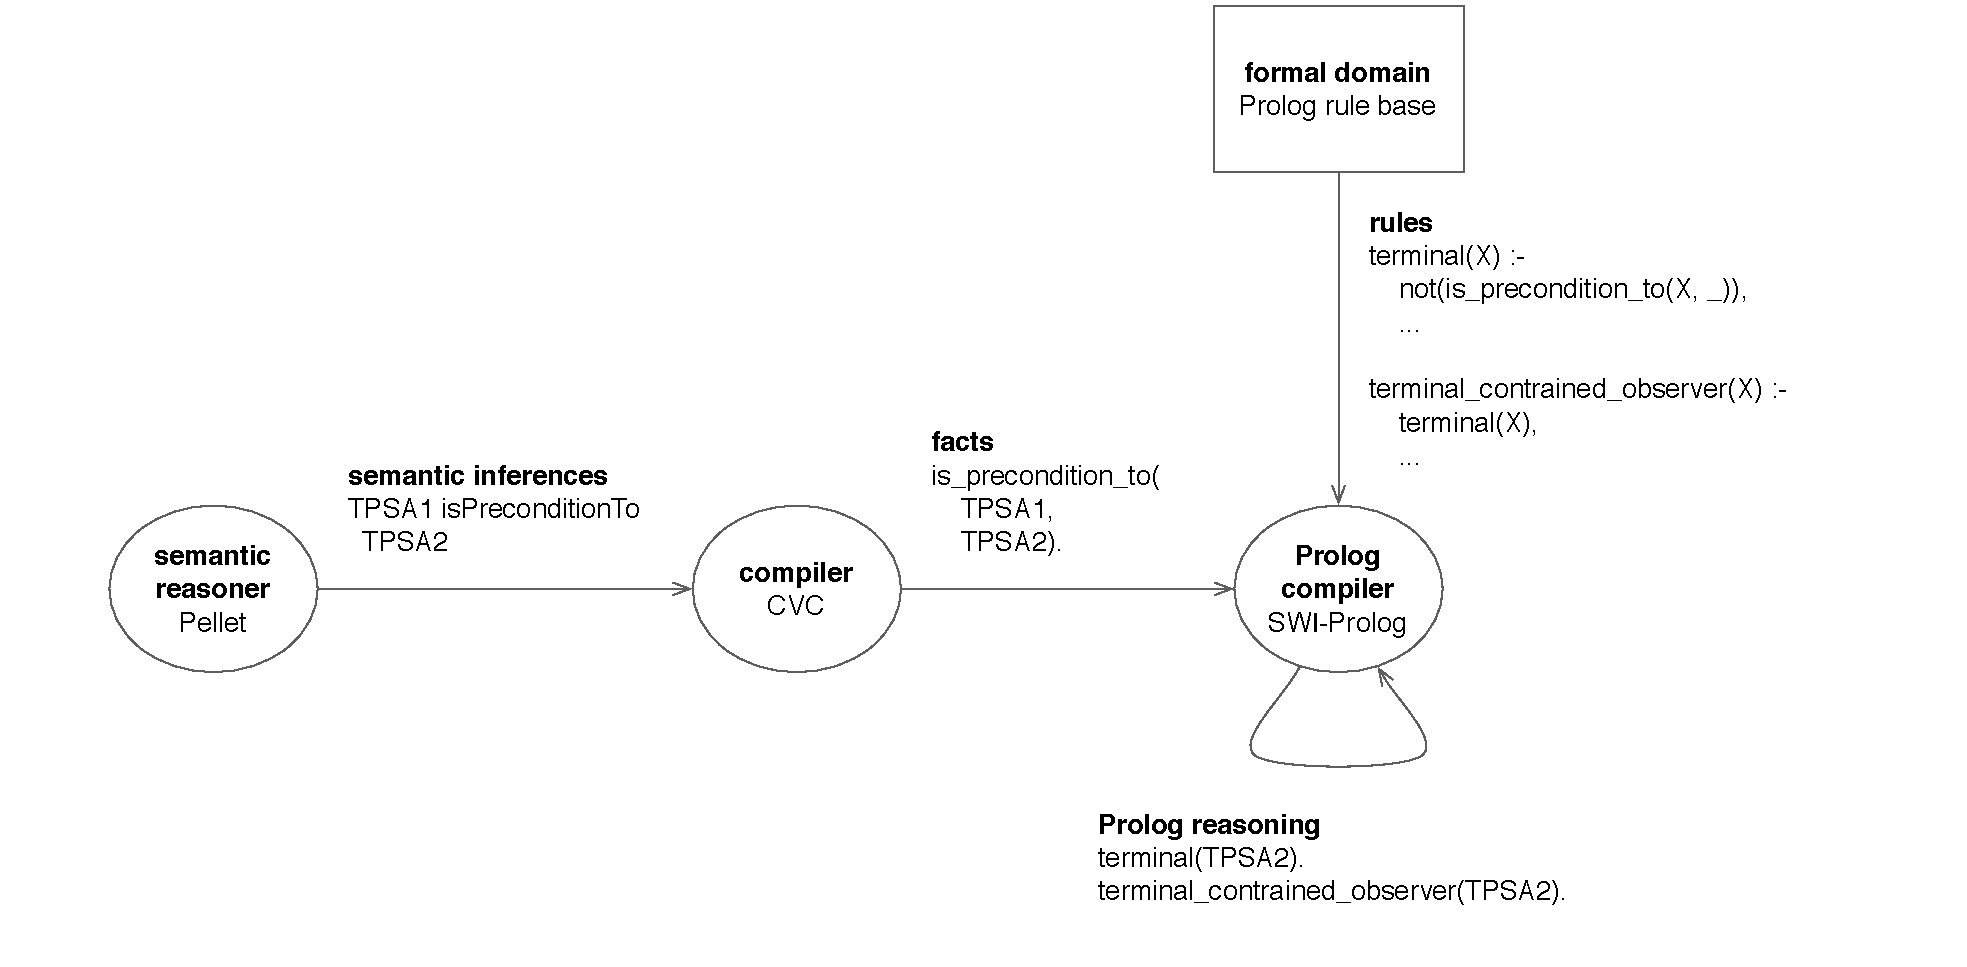
\includegraphics[width=\textwidth]{img/composite-reasoning.pdf}
\caption[Composite reasoning]{Elements of composite semantic- and Prolog-based reasoning with respect to the actions \texttt{TPSA1} and \texttt{TPSA2}; the inferred object property \texttt{isPreconditionTo} presented in Section~\ref{sec:Rule_Based_Modeling}; and the rule \texttt{terminal\_constrained\_observer}.}
\label{fig:composite_reasoning}
\end{figure}

The classification of a kinetic action affects the composition of the PRISM module for the asset to which that action is assigned; for example, the classification of action \texttt{TPSA2} in Mission~A as a \texttt{terminal\_constrained\_observer} affects the PRISM module corresponding to asset~\texttt{H1}. Affected asset module constructs include the action label of the command associated with \texttt{TPSA2} (recall that each asset module command is associated with a specific kinetic action) and, potentially, the action label of the last module command (see inferred arguments in Section~\ref{sec:Behavioral_Modeling}). Kinetic action classifications also generate mission properties; for example, as the last kinetic action to be executed by an asset, the successful execution of a \texttt{terminal\_constrained\_observer} is a desired mission property because it guarantees the successful execution of all preceding actions.

Table~\ref{tab:kinetic_action_classifications} highlights the impact of kinetic action classifications with respect to synthesized DTMC and PCTL constructs. For example, the action label of the asset module command associated with a \texttt{default} classification would assume the value of the identifier assigned to the classified action (as denoted by the dot notation); the action label of the command associated with a \texttt{terminal\_constrained\_observer} classification would assume the identifier of the asset to which the classified action is assigned; and, given the notation in Listing~\ref{lst:PCTL_action_duration_template}, the identifier of the property associated with a \texttt{terminal\_constrained\_observer} classification would assume the value of the identifier assigned to the classified action. Not applicable (n/a) and \texttt{null} values in Table~\ref{tab:kinetic_action_classifications} denote classifications that either do not affect the synthesis of a specific action label, or synthesize an empty action label, respectively. Thus Prolog inferences affect the synthesis of action labels, which in turn impact module synchronization (as described in Section~\ref{sec:Behavioral_Modeling}) and, ultimately, the verification results returned by PRISM\@.

\begin{sidewaystable}
	\centering
	\arrayrulecolor{Gray}
	\renewcommand*\arraystretch{1.3}
	\begin{tabular}{ l | l l | l }
		& \multicolumn{2}{ c | }{\textbf{DTMC asset module}} & \multicolumn{1}{ c }{\textbf{PCTL}}\\
		kinetic action classification & action label & last action label & property id\\
		\hline
		\texttt{default} & \texttt{action.id} & n/a & n/a\\
		\texttt{default\_singleton} & \texttt{action.id} & \texttt{null} & \texttt{action.id}\\
		\texttt{default\_terminal} & \texttt{action.id} & \texttt{null} & \texttt{action.id}\\
		\texttt{subject\_precondition} & \texttt{primary\_asset.id} & n/a & n/a\\
		\texttt{observer\_precondition} & \texttt{primary\_asset.id} & n/a & n/a\\
		\texttt{constrained\_subject} & \texttt{primary\_asset.id} & n/a & n/a\\
		\texttt{leading\_subject} & \texttt{action.id} & n/a & n/a\\
		\texttt{singleton\_subject} & \texttt{primary\_asset.id} & \texttt{primary\_asset.id} & n/a\\
		\texttt{terminal\_subject} & \texttt{primary\_asset.id} & \texttt{primary\_asset.id} & n/a\\
		\texttt{default\_observer} & \texttt{action.id} & n/a & n/a\\
		\texttt{terminal\_observer} & \texttt{action.id} & \texttt{null} & \texttt{action.id}\\
		\texttt{terminal\_constrained\_observer} & \texttt{action.asset.id} & \texttt{action.asset.id} & \texttt{action.id}\\
		\texttt{observer\_and\_constrained\_subject} & \texttt{primary\_asset.id} & n/a & n/a\\
		\texttt{observer\_and\_singleton\_subject} & \texttt{primary\_asset.id} & \texttt{primary\_asset.id} & n/a\\
		\texttt{observer\_and\_terminal\_subject} & \texttt{primary\_asset.id} & \texttt{primary\_asset.id} & n/a\\
		\texttt{subject\_constraint} & \texttt{primary\_asset.id} & n/a & n/a\\
		\texttt{terminal\_subject\_constraint} & \texttt{primary\_asset.id} & \texttt{primary\_asset.id} & \texttt{action.id}\\
	\end{tabular}
	\captionsetup{width=0.7\textwidth}
	\caption[Kinetic action classifications for DTMC and PCTL constructs]{Kinetic action classifications, which are ultimately derived via Prolog inferences, and their impact on synthesized DTMC and PCTL constructs associated with classified actions.}
	\label{tab:kinetic_action_classifications}
\end{sidewaystable}

For several kinetic action classifications, action labels assume the identifier of a \emph{primary asset} (as illustrated in Table~\ref{tab:kinetic_action_classifications}), which may be different from the asset to which a classified action is assigned. The behavioral modeling process described in Section~\ref{sec:Behavioral_Modeling} was guided by two concerns. Our primary goal was to develop template models and properties that could support the verification of multiple and variable UAV mission plans. It was also our intention to accurately model domain processes and thereby achieve the greatest possible confidence in the resulting verification process. To mimic real-world asset behavior, module executions were loosely coupled and synchronizations limited to occur on an as-needed basis. But this approach is not appropriate for modeling cross-cutting actions, which must be verified with temporal precision to ensure kinetic action workflow continuity during asset operations (this issue will be elaborated in Chapter~\ref{chap:Evaluation}). The conflict between modeling and analytical accuracy occurs because enabled DTMC commands are executed by PRISM with equal probability~\cite{PRISM_2010}. Lack of native scheduling precision necessitates the synchronization of all modules representing concepts related to cross-cutting actions. The required synchronization is achieved with the designation, via Prolog inferences, of a single primary asset whose identifier is assumed by the action labels associated with cross-cutting actions.

The Prolog code in Listing~\ref{lst:Prolog_rule_primary_asset} formally defines rule \texttt{primary\_asset}, which encapsulates inferred ontological knowledge encoded with the atoms \texttt{observer\_asset} (line~2), \texttt{observed\_asset} (line~4) and \texttt{observes} (lines~6 and~7). Rule \texttt{primary\_asset} formalizes the concept of a primary asset as an \emph{observer asset} (i.e., an asset observing other assets) that is either not itself observed by, or participates in a symmetric observer relationship with, another asset (a symmetric relationship is the opposite of the asymmetric relationship described in Section~\ref{sec:Modeling_Tactical_Missions}).

\begin{figure}[ht]
\begin{lstlisting}[caption={Prolog code for rule \texttt{primary\_asset}},label=lst:Prolog_rule_primary_asset]
primary_asset(A) :-
    observer_asset(A),
    (
        not(observed_asset(A));
        (
            observes(A, B),
            observes(B, A)
        (*)*)
    (*).*)
\end{lstlisting}
\end{figure}

Lines~1--3 in Listing~\ref{lst:OWL_class_ObserverAsset} formally define class \texttt{ObserverAsset}, which extends class \texttt{Asset}. Every member of class \texttt{ObserverAsset} must be associated via the object property \texttt{hasAction} with a member of class \texttt{Observer}. Lines~5 and~6 formally define the OWL class \texttt{Observer}, which is augmented by a synonymous SWRL rule (lines~8--13). Rule \texttt{Observer} formalizes the concept of an \emph{observer action} as an action that observes cross-cutting actions via preconditions. Given the domain knowledge encoded in Listing~\ref{lst:OWL_class_ObserverAsset}, an observer asset can be described more precisely as an asset that observes other assets via an assigned action that has as precondition a cross-cutting action. Conversely, an \emph{observed asset} is an asset observed by other assets via an assigned cross-cutting action. Class \texttt{ObservedAsset}, which formalizes the observed asset concept, is encoded in a similar manner to class \texttt{ObserverAsset}. Knowledge inferred by Pellet with respect to \texttt{ObserverAsset} and \texttt{ObservedAsset} is transformed by the CVC into knowledge encoded with the Prolog atoms \texttt{observer\_asset} and \texttt{observed\_asset}, respectively.

\begin{figure}[ht]
\begin{lstlisting}[caption={OWL+SWRL code for class \texttt{ObserverAsset}},label=lst:OWL_class_ObserverAsset]
Class: ObserverAsset
  EquivalentTo: Asset
    and (hasAction some Observer)

Class: Observer
  SubClassOf: Action

Rule:
    hasAction(?a, ?x),
    hasAction(?b, ?y),
    hasPrecondition(?y, ?x),
    DifferentFrom (?a, ?b)
  -> Observer(?y)
\end{lstlisting}
\end{figure}

Listing~\ref{lst:OWL_object_property_observes} formally defines the object property \texttt{observes} (lines~1--5), which is augmented by a synonymous SWRL rule (lines~7--12). Rule \texttt{observes} uses the cross-cutting action relationship (lines~8--11) to underpin an asset-oriented subject-observer relationship. Knowledge inferred by Pellet with respect to the OWL concept \texttt{observes} is transformed by the CVC into knowledge encoded with the Prolog atom \texttt{observes}, which is used in the context of rule \texttt{primary\_asset} to formalize a symmetric observer relationship. In conjunction with the observed and observer asset concepts, the \emph{observes} concept supports SWI-Prolog inferences with respect to \texttt{primary\_asset}, which in turn supports kinetic action classifications.

\begin{figure}[ht]
\begin{lstlisting}[caption={OWL+SWRL code for the object property \texttt{observes}},label=lst:OWL_object_property_observes]
ObjectProperty: observes
  Characteristics: Asymmetric,
    Irreflexive
  Domain: Asset
  Range: Asset

Rule:
    hasAction(?a, ?x),
    hasAction(?b, ?y),
    hasPrecondition(?y, ?x),
    DifferentFrom (?a, ?b)
  -> observes(?a, ?b)
\end{lstlisting}
\end{figure}

Rule \texttt{primary\_asset} enables Prolog to discover the assets with assigned cross-cutting actions that have temporal precedence in a workflow of related actions. Such a workflow may comprise one or, given the symmetric observer relationship encapsulated in \texttt{primary\_asset}, multiple primary assets. The action label identifier resulting from a single primary asset guarantees the synchronization of all modules representing concepts related to cross-cutting actions. Synchronization is also guaranteed with multiple primary assets when a single identifier is chosen randomly from the candidate set. We note that a single mission plan comprising multiple independent action workflows could be verified by PRISM without the need for synchronization between the actions that constitute those workflows.

The primary asset mechanism may be perceived as an obfuscated method for achieving what is in essence a random result, at least with respect to a subset of the mission space. But primary assets support an inference-based selection process that is conceptually compatible with the methods that derive the remaining action- and asset-based identifiers in Table~\ref{tab:kinetic_action_classifications}. And while this mechanism fails to eliminate randomness during the identifier selection process, it performs better than random by eliminating and minimizing randomness for mission plans comprising one or more primary assets, respectively. It is of course entirely possible for the primary asset concept, and the reasoning that it affords, to be extended or repurposed in subsequent versions of our prototype. In any case, these concerns apply neither to our method nor our prototype as a whole, but rather to a small subset of the domain model that constitutes our prototype.

As a prelude to the following section, which presents synthesized PRISM artifacts, Table~\ref{tab:Mission_A_classifications} lists kinetic action classifications for the path segment traversal actions specified in Mission~A (top), and the impact of each classification on the synthesized DTMC and PCTL constructs associated with the classified action (bottom).

\newcommand{\true}{\textcolor{green}{true}}
\newcommand{\false}{\textcolor{red}{false}}

\begin{table}[ht]
	\arrayrulecolor{Gray}
	\renewcommand*\arraystretch{1.3}
	\begin{tabularx}{\textwidth}{
			>{\raggedright\hsize=0.56\hsize}X|
			>{\centering\hsize=0.11\hsize}X
			>{\centering\hsize=0.11\hsize}X
			>{\centering\hsize=0.11\hsize}X
			>{\centering\hsize=0.11\hsize}X
		}
		& \texttt{TPSA1} & \texttt{TPSA2} & \texttt{TPSA3} & \texttt{TPSA4}\tabularnewline
		\hline
		\texttt{default} & \false & \false & \false & \false\tabularnewline
		\texttt{default\_singleton} & \false & \false & \false & \false\tabularnewline
		\texttt{default\_terminal} & \false & \false & \false & \false\tabularnewline
		\texttt{subject\_precondition} & \false & \false & \false & \false\tabularnewline
		\texttt{observer\_precondition} & \true & \false & \false & \false\tabularnewline
		\texttt{constrained\_subject} & \false & \false & \true & \false\tabularnewline
		\texttt{leading\_subject} & \false & \false & \false & \false\tabularnewline
		\texttt{singleton\_subject} & \false & \false & \false & \false\tabularnewline
		\texttt{terminal\_subject} & \false & \false & \false & \false\tabularnewline
		\texttt{default\_observer} & \false & \false & \false & \false\tabularnewline
		\texttt{terminal\_observer} & \false & \false & \false & \false\tabularnewline
		\texttt{terminal\_constrained\_observer} & \false & \true & \false & \false\tabularnewline
		\texttt{observer\_and\_constrained\_subject} & \false & \false & \false & \false\tabularnewline
		\texttt{observer\_and\_singleton\_subject} & \false & \false & \false & \false\tabularnewline
		\texttt{observer\_and\_terminal\_subject} & \false & \false & \false & \false\tabularnewline
		\texttt{subject\_constraint} & \false & \false & \false & \false\tabularnewline
		\texttt{terminal\_subject\_constraint} & \false & \false & \false & \true\tabularnewline
		\hline\hline
		asset module action label & \texttt{H1} & \texttt{H1} & \texttt{H1} & \texttt{H1}\tabularnewline
		asset module last action label & n/a & \texttt{H1} & n/a & \texttt{H1}\tabularnewline
		property id & n/a & \texttt{TPSA2} & n/a & \texttt{TPSA4}\tabularnewline
	\end{tabularx}
	\caption[Kinetic action classifications for Mission~A]{Kinetic action classifications for the path segment traversal actions specified in Mission~A (top), and the impact of each classification on the synthesized DTMC and PCTL constructs associated with the classified action (bottom).}
	\label{tab:Mission_A_classifications}
\end{table}

\section{Synthesized Models and Properties}
\label{sec:Synthesized_Models_and_Properties}

The CVC uses explicit and inferred domain knowledge to synthesize DTMC and PCTL artifacts from predefined templates; for example, the asset module template presented in Section~\ref{sec:Behavioral_Modeling} underpins the synthesis of one module per each asset in Mission~A\@. The PRISM code in Listing~\ref{lst:PRISM_asset_module_code} specifies a synthesized asset module corresponding to asset~\texttt{H2}, where the commands in lines~3 and~4 represent, respectively, the execution of actions~\texttt{TPSA3} and~\texttt{TPSA4} assigned to~\texttt{H2}.

\begin{figure}[ht]
\begin{lstlisting}[caption={PRISM asset module code},label=lst:PRISM_asset_module_code]
module Hummingbird2
  e2 : [0..120] init 120;
  [H1] e2>0 & d3>0 -> (e2'=e2-1);
  [H1] e2>0 & d4>0 -> (e2'=e2-1);
  [H1] e2=0 | d4=0 -> true;
endmodule
\end{lstlisting}
\end{figure}

As a consequence of the realization-based inferences described in Section~\ref{sec:Verification_with_Semantic_Reasoning}, the CVC synthesizes an asset survivability module to calculate the probability of survival for~\texttt{H2} (as described in Section~\ref{sec:Modeling_Survivability}). The PRISM code in Listing~\ref{lst:PRISM_asset_survivability_code} specifies the synthesized survivability module corresponding to asset~\texttt{H2}, where variable~\texttt{a2d} (lines~6--8) represents the asset's destruction.

\begin{figure}[ht]
\begin{lstlisting}[caption={PRISM asset survivability code},label=lst:PRISM_asset_survivability_code]
const int start4 = 60;
const int finish4 = 0;
formula actn4_tai = d4>finish4 & d4<=start4;

module Hummingbird2_Survivability
  a2d : bool init false;
  [H1] !a2d & (*\hspace{1.8mm}*)actn4_tai -> 0.99:(a2d'=false) + 0.01:(a2d'=true);
  [H1] (*\hspace{1.8mm}*)a2d | !actn4_tai -> true;
endmodule
\end{lstlisting}
\end{figure}

The CVC also synthesizes PRISM code to calculate a RAF value for the threat area incursion prosecuted by asset~\texttt{H2} (as described in Section~\ref{sec:Modeling_Risk_Acceptability}). The PRISM code in Listing~\ref{lst:PRISM_risk_acceptability} specifies the synthesized sensor action counter module corresponding to asset~\texttt{H2}. Variables \texttt{start4}, \texttt{finish4} and \texttt{actn4\_tai} in Listing~\ref{lst:PRISM_risk_acceptability} are declared in Listing~\ref{lst:PRISM_asset_survivability_code}.

\begin{figure}[ht]
\begin{lstlisting}[caption={PRISM risk acceptability code},label=lst:PRISM_risk_acceptability]
formula duration4 = start4 - finish4;

formula tkad2 = duration4;

module SensorActionCounter2
  sad2 : [0..tkad2] init 0;
  [H1] (*\hspace{1.8mm}*)actn4_tai &(*\hspace{1.8mm}*) (r5) & sad2<tkad2 -> (sad2'=sad2+1);
  [H1] !actn4_tai | !(r5) -> true;
endmodule

formula raf2 = sad2 / tkad2;
\end{lstlisting}
\end{figure}

At the conclusion of the synthesis process, the DTMC artifact that models Mission~A is verified against a set of synthesized PCTL properties. The PRISM code in Listing~\ref{lst:PRISM_mission_property} specifies a synthesized property for Mission~A\@. This property comprises variables~\texttt{d2} and~\texttt{d4}, which represent the durations of~\texttt{TPSA2} and~\texttt{TPSA4}, respectively; variable \texttt{a2d}, described above; and variable~\texttt{raf2}, which represents the RAF value for the threat area incursion committed by asset~\texttt{H2}. The property need not comprise variables to represent the durations of~\texttt{TPSA1} and~\texttt{TPSA3} because these actions precede~\texttt{TPSA2} and~\texttt{TPSA4}, respectively. In other words, the successful execution of~\texttt{TPSA1} is implied by the successful execution of~\texttt{TPSA2} (this implication is denoted by the classification of \texttt{TPSA2} as a \texttt{terminal\_constrained\_observer}), etc.

\begin{figure}[ht]
\begin{lstlisting}[caption={PRISM mission property code},label=lst:PRISM_mission_property]
P=? [ F d2=0 & d4=0 & !a2d & raf2>0.6(*\hspace{1.8mm}*)]
\end{lstlisting}
\end{figure}

Given the property in Listing~\ref{lst:PRISM_mission_property}, the probability of success for Mission~A is calculated by PRISM to be approximately 0.299. In particular, the verification of Mission~A assigns variables~\texttt{d2} and~\texttt{d4} with values of zero; variable~\texttt{!a2d} is assigned a probability of approximately 0.299; and variable~\texttt{raf2} is assigned a value of approximately 0.833.

\section{Implementation}
\label{sec:Implementation}

We have implemented several of the components that constitute our prototype. The ontology described in Section~\ref{sec:Semantic_Modeling} and Section~\ref{sec:Rule_Based_Modeling} was implemented in OWL+SWRL\@. The Prolog rule-base described in Section~\ref{sec:Rule_Based_Modeling} was implemented in SWI-Prolog. The DTMC and PCTL templates presented in Section~\ref{sec:Behavioral_Modeling} were implemented in the programming language Ruby (version 1.9.3). And the DSL described in Section~\ref{sec:High_Level_Specifications_in_YAML} was implemented in YAML, which is particularly compatible with Ruby. Because of its powerful reflective and meta-programming capabilities, Ruby affords our prototype flexibility to substitute the current YAML DSL with a more expressive mission specification language, if so required~\cite{Flanagan_2008,Perrotta_2010}.

In developing the prototype, we leveraged open source software including Pellet 2.2.0, PRISM 4.1 and the Prot\'{e}g\'{e} ontology editor (version 4.1.0). While integration, testing and extension of implemented components is currently ongoing, completed work was sufficient to support an evaluation, which is presented in Chapter~\ref{chap:Evaluation}.

\section{Related Work}
\label{sec:Cascading_Verification_Related_Work}

Cascading verification can be considered a form of semantic model checking, which has been studied exclusively in the context of the Web service domain.

Narayanan and McIlraith encode Web service capability descriptions and behavioral properties with DAML-S and Petri net formalisms, respectively~\cite{Narayanan_2002}. DAML-S is a DAML+OIL ontology for describing Web services. For any given Web service, an implemented system generates the Petri net corresponding to the DAML-S description of that service. The resulting net is used by KarmaSIM, a modeling and simulation environment, to perform various analysis techniques including reachability analysis and deadlock detection.

The model checking algorithm presented by Di Pietro et al.\ uses a DL-based ontology to formalize the Web service domain~\cite{Di_Pietro_2012}. The behavior of each Web service is modeled as a \emph{state transition system} (STS), while behavioral requirements are encoded with CTL\@. Both STS and CTL formalisms are extended with semantic annotations. For any given Web service, the algorithm generates a finite STS corresponding to the annotated description of that service. The resulting model is verified with model checking. The same algorithm is used by Boaro et al.\ to verify Web service security requirements~\cite{Boaro_2010}.

Oghabi et al.\ use OWL-S, an OWL ontology that supersedes DAML-S, to describe Web service behavior~\cite{Oghabi_2011}. For any given Web service, an implemented system generates a PRISM model corresponding to the OWL-S description of that service. The resulting model is verified with PRISM\@. Ankolekar et al.\ translate OWL-S process models to equivalent PROMELA models, which are verified with the SPIN model checker~\cite{Ankolekar_2005}. Liu et al.\ extend OWL-S with multiple annotation layers for specifying Web service flow properties including temporal constraints~\cite{Liu_2008}. Annotated OWL-S models are transformed to corresponding \emph{time constraint Petri net} (TCPN) models, which are verified with model checking. Lomuscio and Solanki express OWL-S process models with the \emph{interpreted systems programming language} (ISPL)~\cite{Lomuscio_2009}. ISPL is the system description language for MCMAS, a symbolic model checker tailored to the verification of multi-agent systems. In this context, Web services and Web service compositions are viewed as agents and multi-agent systems, respectively.

Our method is perhaps most compatible with the work presented by Oghabi et al. Similarities include the motivation to verify stochastic behavior and the development of a system that synthesizes PRISM models from OWL knowledge. But unlike our prototype, the system developed by Oghabi et al.\ does not synthesize behavioral properties, nor does it exploit inferred knowledge to support the synthesis of DTMC artifacts. Inferred knowledge is utilized in other work including that of Narayanan and McIlraith, Di Pietro et al.\ and Boaro et al. But existing work is exclusively concerned with the verification of Web services, and does not address the expressive and reasoning limitations that constrain OWL\@. The work presented in this thesis is (to our knowledge) unique because it addresses semantic model checking limitations, and applies the resulting method to a novel domain.

\section{Summary}
\label{sec:Cascading_Verification_Summary}

Chapter~\ref{chap:Domain_Modeling} describes the technologies and modeling methods that underpin cascading verification; in this chapter, we describe the actual verification process, which involves several stages of reasoning and analysis. The process begins when model builders use a high-level DSL to encode system specifications. A compiler uses automated reasoning to verify the consistency between each specification and formalized domain knowledge encoded in OWL+SWRL and Prolog. If consistency is deduced, then explicit and inferred domain knowledge is used by the compiler to synthesize a system model and behavioral properties from template code. PRISM subsequently verifies the model against the properties.

At its core, this chapter exposes the composite inference mechanism that underpins our method and prototype. Composite reasoning encompasses Pellet- and Prolog-based inference services; the former include consistency checking and realization with respect to an OWL+SWRL ontology, while the latter involve query resolution with respect to a knowledge base comprising rules and facts. Prolog-based inferences enable our prototype to classify kinetic actions, and thereby calibrate the synthesis of PRISM modules related to those actions. Our implementation of composite reasoning is illustrated with several examples in the context of Mission~A, which is assumed to involve the prosecution of a threat area incursion. The discussion in this chapter thus utilizes the tactical case study introduced in Section~\ref{sec:Modeling_Tactical_Missions}.

By tracing cascading verification from system specifications to probabilistic model checking, we describe a prototype greater than the sum of its parts, i.e., a prototype that integrates technologies presented in Chapter~\ref{chap:Domain_Modeling} to improve the correctness of UAV mission plans. The following chapter quantifies this improvement.
